%
% File acl2014.tex
%
% Contact: koller@ling.uni-potsdam.de, yusuke@nii.ac.jp
%%
%% Based on the style files for ACL-2013, which were, in turn,
%% Based on the style files for ACL-2012, which were, in turn,
%% based on the style files for ACL-2011, which were, in turn, 
%% based on the style files for ACL-2010, which were, in turn, 
%% based on the style files for ACL-IJCNLP-2009, which were, in turn,
%% based on the style files for EACL-2009 and IJCNLP-2008...

%% Based on the style files for EACL 2006 by 
%%e.agirre@ehu.es or Sergi.Balari@uab.es
%% and that of ACL 08 by Joakim Nivre and Noah Smith

\documentclass[11pt]{article}
\usepackage{acl2014}
\usepackage{times}
\usepackage{url}
\usepackage{latexsym}
\usepackage{tabulary}
\usepackage{tabulary}
\usepackage{comment}
\usepackage{graphicx}
\usepackage{array}
\usepackage{multirow}

%\setlength\titlebox{5cm}

% You can expand the titlebox if you need extra space
% to show all the authors. Please do not make the titlebox
 % smaller than 5cm (the original size); we will check this
% in the camera-ready version and ask you to change it back.

\title{Toward Macro-Insights  for Suicide Prevention: \\ Analyzing Fine-Grained Distress at Scale}

%\author{Ravdeep Johar\\
 % Department of Computer Science \\
 % Rochester Institute of Technology \\
 % {\tt rsj7209@rit.edu} \And
 %Christopher M. Homan\\
 % Department of Computer Science \\
 % Rochester Institute of Technology \\
  %{\tt cmh@cs.rit.edu}\\\\ 
 %}

\date{March 21, 2014}

\begin{document}
\maketitle
\begin{abstract}
Suicide is a leading cause of death in the United States and one that has grown to nearly epidemic proportions in some communities. One of the major challenges to suicide prevention is that those who may be most at risk cannot be relied upon to report their condition to clinical practice. This paper takes an initial step toward the automated detection of suicidal risk factors through social media activity, with no reliance on self-reporting.  We consider the performance of annotators with various degrees of expertise in suicide prevention at annotating microblog data for the purpose of training text-based models for detecting suicide risk behaviors.
 \end{abstract}

\section{Introduction}


Suicide is among the leading causes of death for individuals 10--44 years of age in the United States \cite{heron2009deaths}. Indeed, while mortality rates for most illnesses decreased between 2008 and 2009, the rate of suicide increased by 2.4\%  \cite{heron2009deaths}. The lifetime prevalence for suicidal ideation is 5.6--14.3\% in the general population, and as high as 19.8--24.0\% among youth~\cite{nock2008suicide}. 

The first step toward suicide \emph{prevention} is to identify, ideally in consultation with clinical experts, the risk factors associated with suicide.  Due to social stigma among other sociocultural factors~\cite{crosby2011self}, individuals with suicidal ideation may not always reach out to professionals or, if they do, provide them with accurate information. They may not even realize their own level of suicide risk before it is too late. Self-reporting, then, is not an entirely reliable means of detecting and assessing suicide risk, and research on suicide prevention can benefit from also exploring other data sources.

 Individuals may be more inclined to seek support from informal resources, such as social media, instead of seeking treatment (Crosby et al., 2011; Bruffaerts et al., 2011; Ryan et al., 2010). Evidence suggests that youth and emerging adults usually prefer to seek help from their friends and families; however, higher levels of suicidal ideation are associated with lower levels of help-seeking from both formal or informal resources (Deane et al., 2001).  

These trends in help-seeking behavior suggests that social media might be a rich outlet for learning about support seeking.
Internet- and telecommunications-driven activity is revolutionizing the social sciences by providing data---much of it publicly available---on human activity in situ, at volumes and a level of time and space granularity never before approached. Can such data improve clinical preventative study and measures by providing access to at-risk individuals who would otherwise go undetected, and by leading to better science about suicide risk behaviors? 

\newcite{mann1999toward} developed the stress diathesis model for suicidal behavior, using many of the aforementioned risk factors.  This model suggests (1) that objective states, such as depression or life events, as well as subjective states and traits, such as substance abuse or family history of depression, suicide, or substance abuse, were among the risk factors that contributed to suicidal ideation, and (2) that the presence of these factors could eventually lead to either externalizing (e.g., interpersonal violence) or internalizing aggression (e.g., attempting suicide).

	Since the stress-diathesis model was developed using risk factors for suicidal behavior and because it makes a connection between internalized and externalized acts, it is a suitable framework to analyze publicly available linguistic data from social media outlets such as Twitter. Data from social media can be used as a natural experiment to examine depression and suicidal ideation without being constrained by such sample biases as the willingness of individuals to take part in research and/or seek out formal sources of support. Moreover, this natural experiment method may provide information about individuals who are unlikely to engage in formal help-seeking behaviors and eventually could be used to identify effective methods of natural helping. Hence, this macro-level approach to monitoring suicidal behaviors may have future implications not only for identifying individuals who have a higher prevalence for suicidal behaviors but it could eventually lead to additional methods for enhancing protective factors against suicide.  

In this paper, we take steps toward the automatic detection of suicide risk among individuals via social media. We use methods that take advantage of lexical analysis to retrieve microblog posts (tweets) from Twitter and compare the performance of human annotators---some being experts, and some not---to rate the level of \emph{distress} of each tweet. According to \newcite{nock2010measuring} distress is an important risk factor in suicide, and one that is observeable from microblog text, though admittedly observing suicide risk behavior is a subjective and noisy venture.  \emph{Clinical} expert annotation, rather than general-purpose tools for content and sentiment analysis such as LIWC (Linguistic Inquiry and Word Count), provides a basis for text-based statistical modeling.
% that is free of the sort of self-reporting biases that plague suicidality. 
We also show that expertise-based keyword retrieval, departing from knowledge about contributing risk factors, results in better interannotater agreement in both novice-novice and novice-expert annotation when the keywords reflect the task at hand.


\section{Related Work}
Data on suicide traditionally comes from healthcare organizations, large-scale studies, or self reporting \cite{crosby2011self,horowitz2009suicide}. These sources are limited by sociocultural barriers, such as stigma and shame, among other reasons \cite{crosby2011self}. Moreover, suicide is a fundamentally subjective, complex phenomenon with a low base rate. For these reasons, data on suicide is never particularly reliable and many researchers tend to focus on the relationship between risk factors and suicidal behavior, without relying heavily on theoretical models \cite{nock2008suicide}.

Approximately one-third of all individuals who reported suicidal ideation in their lifetime made a plan to commit suicide. Nearly three-quarters of those who reported making a suicide plan actually attempted suicide \cite{kessler1999prevalence}. According to \newcite{kessler1999prevalence}, the odds of attempting suicide increased exponentially when individuals endorsed three of more risk factors (e.g., having a mood or substance abused disorder). 

Demographics, previous suicide attempts, mental health concerns (i.e., depression, substance abuse, suicidal ideation, self-harm, or impulsivity), family history of suicide, interpersonal conflicts (i.e., family violence or bullying), and mechanism, i.e., means for suicidal behavior (e.g., firearms), are commonly cited risk factors for suicidal behavior \cite{nock2008suicide,crosby2011self,gaynes2004screening,harriss2005suicidal,shaffer2004columbia,shaffer2004columbia,brown2000risk}. 




More broadly in clinical contexts, evidence suggests that when it comes to judgments that involve clinical phenomena, experts and novices behave differently. For example, in a medical image inspection task, \newcite{li2012learning} identified differences in perceptual expertise patterns between novices (students) and clinically trained physicians. Similarly, \newcite{womack2012disfluencies} identified  differences in linguistic behaviors between experienced, attending dermatologists vs.\ resident dermatologists-in-training based on diagnostic verbal narratives. Such distinctions intuitively make sense, as the learning of medical domain knowledge requires advanced education in conjunction with substantial practical field experience. In a task such as medical image inspection, the subtle cues that point an observer to evidence that allow them to identify a clinical condition, while accessible to experts with training and perceptual expertise to guide their exploration, are likely to be missed by novices who lack that background and clinical understanding. Such expertise can then be integrated into human-centered health-IT systems \cite{guo2014infusing}, in order to introduce novel ways to retrieve medical images and take advantage of an understanding of which information is useful. It is reasonable to assume that this knowledge gap also applies to other knowledge-intensive clinical domains such as mental health. In this study, we explore this question and study if novice vs.\ expert annotation makes a difference for identifying distress in social media texts, as well as what the impact of expert vs.\ novice annotation is for subsequent computational modeling with the annotated data.


Affect in language is a phenomenon that has been studied both in speech and in the text analysis domain, as well as in many other modalities \cite{calvodmello2010}. Clearly, emotion is a key element in the human experience, but it is notoriously difficult to pin down and scholars in the affective sciences lack a single agreed-upon definition for emotion. Accordingly, different theoretical constructs have been proposed to describe affect and affect-related behaviors \cite{picard1997}. In addition, research on affect in language has shown that such phenomena tend to be subjective, lack real ground truth (often resulting in moderate kappa scores), and have particularly fuzzy semantics in the gray zone where neutrality and emotion meet \cite{alm08}. These kinds of problem characteristics bring with them their own set of demanding challenges from a computational perspective \cite{alm2011}. Yet, the nature of such problems make them incredibly important to study, despite the challenges involved. 

Level of distress is a key element to consider when evaluating at-risk behaviors with respect to suicidal behavior or depression. \newcite{lehrmanetal2011} conducted a first study on the computational modeling of distress based on short forum texts, yet left many areas wide open for continued study. For example, analysis at scale is one such open issue. More specifically, Pestian and colleagues \cite{pestinaetal2009,pestinaetal2008} used computational methods to understand suicide notes. However, when it comes to preventive contexts, such data are less insightful. For preventive health, access to real time health-related data that dynamically evolves can allow us to address macro-level analysis, and social media texts provide the additional opportunity to model the phenomena of interest at scale.

Sentiment analysis has been widely studied in a number of computational settings, including on various social networking sites. 
A rather substantial body of work already exists on the use of Twitter to study emotion~\cite{bollen2011twitter,dodds2011temporal,wang2012harnessing,pfitzner2012emotional,kim2012you,bollen2011happiness,pfitzner2012emotional,bollen2011modeling,mohammad2012emotional,golder2011diurnal,de2012not,de2012happy,de2013major,de2013understanding,hannak2012tweetin,thelwall2011sentiment,pak2010twitter}. For instance,
Golder and and Macy study aggregate global trends in ``mood,'' and show, among other things, that people wake up in a relatively good mood that decays as the day progresses \cite{golder2011diurnal}, Bollen et al.~\cite{bollen2011modeling} show that tweets from users who took a standard diagnostic instrument for mood are often tied to current events, such as elections and holidays.

Relatively little of this work has focused on suicide or related psychological conditions. \newcite{masuda2013suicide} study suicide on mixi (a Japanese social networking service). \newcite{cheng2012opportunities} consider the ethical and political implications of online data collection for suicide prevention. \newcite{Jay} show correlations between frequency in tweets related to suicide and actual suicide in the 50 United States of America. \newcite{sadilek2014modeling} study depression on Twitter. De Choudhury and collaborators studied depression---in general and post-partem---in Twitter~\cite{de2012not,de2012happy,de2013major,de2013understanding} and Facebook~\cite{de2014characterizing}. \newcite{homan2014social} investigate depression in TrevorSpace. A number of social theories of suicide have been proposed~\cite{wray2011sociology}, but most of this work was with respect to offline social systems. 




\section{Methods}
In this section, we describe the methods we use to label and detect distress in Twitter data. Our process involves four main phases: (1) We filter a corpus, obtained from~\newcite{sadilek2012predicting}, of approximately 2.5 million tweets from 6,237 unique users in the New York City area that were sent during a 1-month period between May and June, 2010, into a set of 2,000 tweets that are relatively likely to be centered around suicide risk factors. (2) We annotated each of these 2,000 tweets with their level of distress, and also analyzed the annotations in detail. (3) We then train support vector machines and topic models with the annotated data, except for a held-out subset of 200 tweets. (4) Finally, we assess the effectiveness of these methods on the held-out set.


\begin{table}[h]
\footnotesize
\begin{tabular}{|c|c|c|}
\hline
\multirow{4}{*}{\begin{tabular}[c]{@{}c@{}}Source\\ tweets\end{tabular}}              &   Number of tweets           &   2,535,706  \\ 
                                                                                    &  Unique geo-active users           &   6,237 \\ 
                                                                                    & ``Follows'' relationships           &  102,739 \\ 
                                                                                    & ``Friends'' relationships &   31,874   \\\cline{1-3} 
\multirow{5}{*}{\begin{tabular}[c]{@{}c@{}}Filtered\\ tweets\end{tabular}}              & Number of tweets              & 2000    \\ 
                                                                                    & Unique users              & 1467    \\ 
                                                                                    & Unique tokens             & 1714167 \\ 
                                                                                    & Unique bigrams             & 9246715 \\
                                                                                    & Unique trigrams             & 13061142 \\ \hline
\multirow{13}{*}{\begin{tabular}[c]{@{}c@{}}Categories\\ distribution\end{tabular}} & LIWC sad                       & 1370    \\ \cline{2-3} 
                                                                                    & Depressive feeling        & 283     \\
                                                                                    & Suicide ideation          & 123     \\ 
                                                                                    & Depression symptoms       & 72      \\ 
                                                                                    & Self harm                 & 67      \\ 
                                                                                    & Family violence/discord   & 47      \\ 
                                                                                    & Bullying                  & 10      \\ 
                                                                                    & Gun ownership             & 10 \\ 
                                                                                    & Drug abuse                & 6       \\ 
                                                                                    & Impulsivity               & 6       \\ 
                                                                                    & Prior suicide attempts    & 2       \\ 
                                                                                    & Suicide around individual & 2       \\ 
                                                                                    & Psychological disorders   & 2       \\ \hline 
                                                                                          
\end{tabular}
\caption {Summary statistics of the and thematic categories distributions of the collected dataset. The data was collected from NYC. Geo-active users are those who geo-tag (i.e., automatically post the GPS location of) their tweets relatively frequently (more than 100 times per month).} 
\label{table::dataset}
\end{table}

\subsection{Filtering tweets}

We first preprocessed each tweet in the corpus by (a) converting all text to lower case; (b) stripping out punctuation and special characters; and (c) building a dictionary of more than 5,400 terms that captured informal Twitter registers, such as abbreviations and netspeak, based on http://www.noslang.com/dictionary. 

In order to test the effectiveness of various methods of capturing useful corpus data, we used two different methods to filter for tweets that are relatively likely to center on suicide risk factors. As the first method, we used the Linguistic Inquiry and Word Count (LIWC) to capture 1,370 tweets by sampling randomly from the all tweets with at least the $2,000$th-highest LIWC sad score. LIWC has been widely used to estimate emotion in online social networks, and specifically to  mood on Twitter. This slight amount of randomness in filtering tweets this way was intended to avoid selecting obvious false positives, such as the use of ``sad'' in nicknames.

Next, we adopted a collection of inclusive search terms/phrases from \cite{Jay}, which was designed specifically for capturing tweets related to suicide risk factors, and applied them to our source corpus. These terms yielded 630 tweets.


\subsection{Novice and Expert Tweet Annotation}
\begin{figure}[h]
  \centering
{\small
\begin{verbatim}
978: Date: XXXX 
    -3: dat man on maury is overreacting
    -2: @XXXX cedes!!! [-0:21:25]
    -1: yesssss! da weatherman was wronq
>>> @XXXX awwww thanks trae-trae
     1: rt @XXXX: abt 2 hop in a kab to 
     2: @XXXX yeaa [+0:03:59]
     3: @XXXX wassup? [+0:05:28]
Msg_id: XXXX  [Distress: ND, LIWC Sad: No]
\end{verbatim}}
  \caption{Example input for annotator. Each line is one tweet. The tweet being annotated is indicated by $>>>$. Annotators were given context in the form of a window of three immediately preceding tweets s well as three immediately following tweets, including their respective time-stamped offsets compared to the annotation target tweet. 
(Tweeter information has been blanked out.)}
  \label{fig:annotateeg}
\end{figure}

We then divided the resulting set of 2,000 filtered tweets (1,370 from the LIWC sad dimension and 630 from suicide-specific search terms), into two randomized sets of 1,000 tweets each. Both sets had the same proportion of LIWC-filtered and suicide-specific-filtered tweets. A novice annotated the first set and a counseling psychologist with experience in suicide related research annotated the second set. A second novice annotated a subset of 250 tweets of the first set, to reveal interannotator agreement between novices as one might expect a novice without training to be less systematic. Each tweet in each set was rated on a four-point scale (H, ND, LD, HD) according to the level of distress evident (Table~\ref{tab:distress}).


\begin{table}[h]
  \centering
  \begin{tabular}[h]{ll}
   \textbf{Code}&\textbf{Distress Level}\\
\hline
 H & happy \\
ND & no distress\\
 LD & low distress\\
HD &high distress
  \end{tabular}
  \caption{Distress-related categories used to annotate the tweets.}
  \label{tab:distress}
\end{table}


For the annotation process itself, each tweet was provided with a context, i.e., three tweets before and after the tweet to be annotated, along with the timestamp of these tweets and thematic category to which the tweet belonged (Figure~\ref{fig:annotateeg}).






\subsection{Modeling}
We represent each tweet as a collection of  all unigrams, bigrams, and trigrams in the message. For example, a simple tweet ``I am so happy'' is represented as the following \emph{feature vector}: \{I, am, so, happy, I am, am so, so happy, I am so, am so happy\}. This method allows one to construct prior probabilities on pairs and triples of consecutive words and thus model the probability spaces of arbitrarily long utterances, in a way that is natural and often effective in representing linguistic data with at least a limited context (given data sparsity concerns for longer sequences) for the purpose of classification or topic modeling.



We perform topic modeling on our dataset to compare the topics. Topic modeling is often used to analyze text data by finding topics within a corpus of documents. A topic is characterized by lexical items that are likely to occur with the topic. These models are capable of connecting words with similar meanings and distinguish words with multiple meanings. We utilize  Latent Dirichlet Algorithm (LDA) \cite{Blei} to create these topics. In this method the documents (in our case tweets) are represented as random mixtures over latent topic where each topic is characterized by a distribution over words. Before performing the topic modeling, the stop words and words that occur only once in the dataset are removed. The LDA algorithm then establishes three topics using $100$ iterations. 

We use Support Vector Machines (SVM), a machine learning method that is used to train a classification model that can assign class labels to previously unseen tweets, to assess the power of our annotations. SVMs treat each tweet as a point in an extremely high dimensional space (one dimension per uni-, bi-, and trigram in the corpus). SVMs are a form of \emph{linear separator}. They have proven to be an extremely effect tool in classifying text in numerous settings, for different types of problems and with varying form of text data, including Twitter. 


\section{Results}


\begin{figure}[h]
\centering
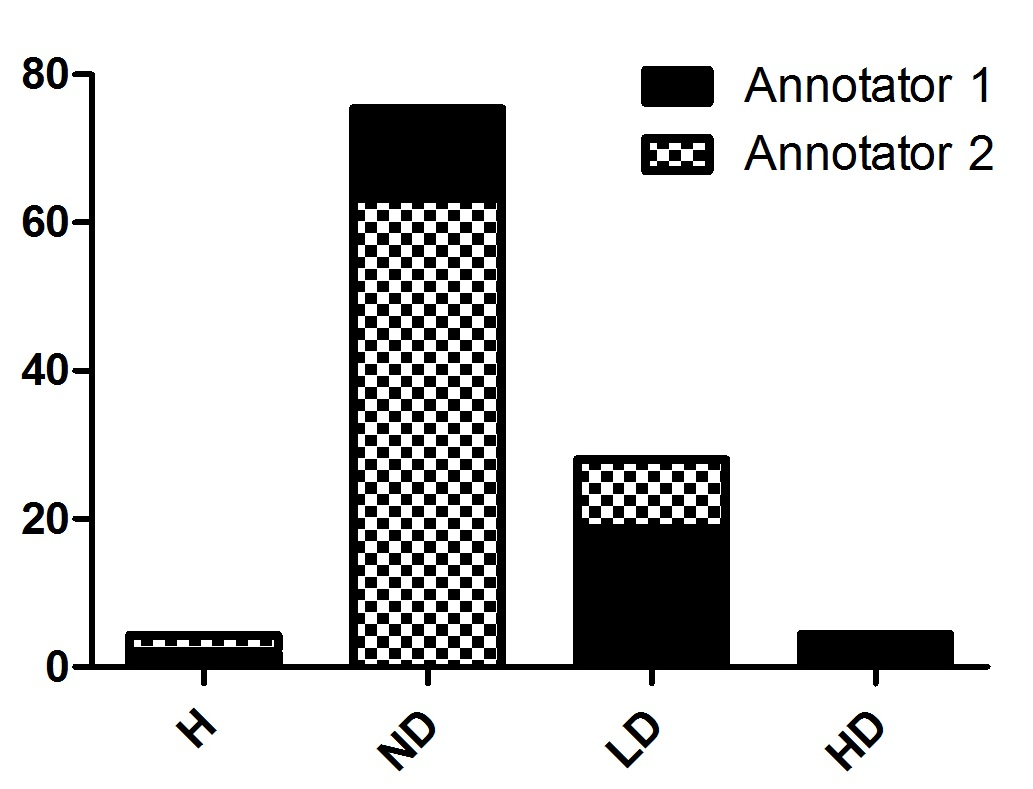
\includegraphics[scale=0.65]{ChrisCissi4cat.jpg}
\caption{Distribution of distress level annotations on the tweets annotated by Novices 1 and 2 (N=250, identical set).}
\label{fig:distress-distrib1}
\end{figure}

\begin{figure}[h]
\centering
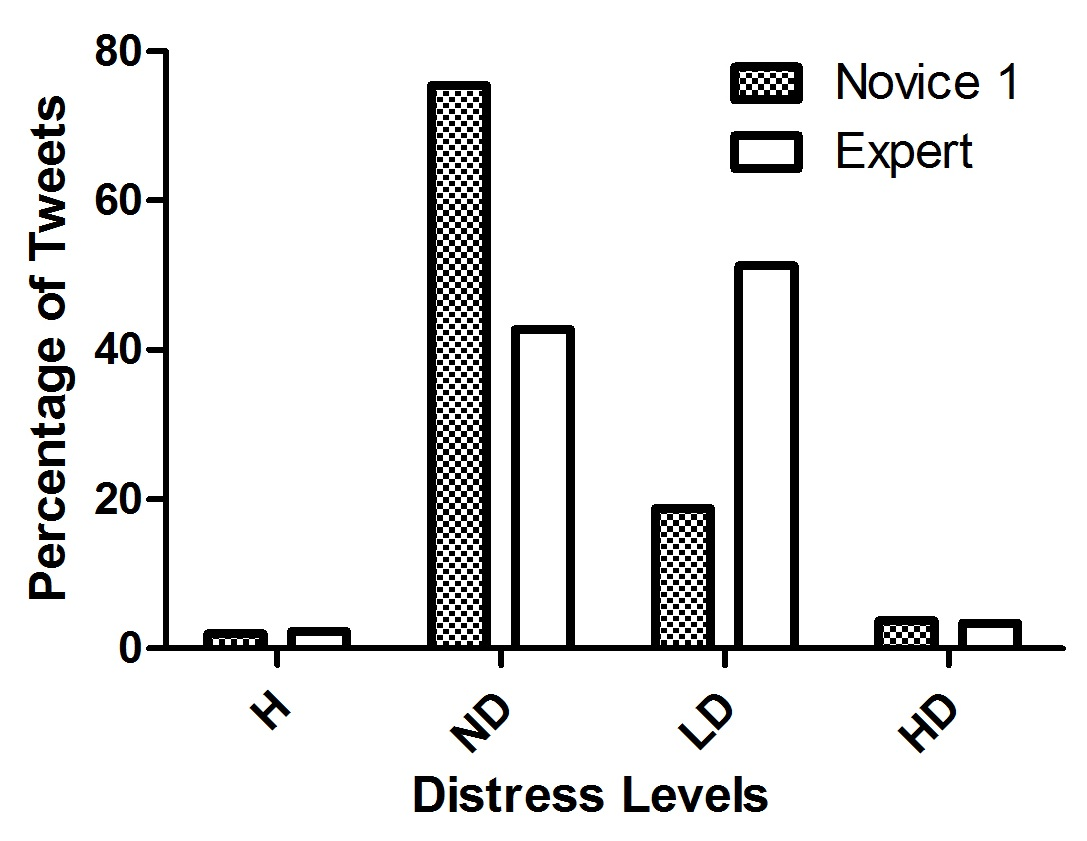
\includegraphics[scale=0.65]{ChrisMegan4Cat.jpg}
\caption{Distribution of distress level annotations from Novice 1 and Expert. Note the these two datasets are disjoint (N = 1000 tweets, respectively).}
\label{fig:distress-distrib2}
\end{figure}

Figure \ref{fig:distress-distrib1} shows the distribution of annotation labels for the subset of tweets that Novices 1 and 2 both annotated, and Figure \ref{fig:distress-distrib2} compares the overall annotation distributions between Novice 1 and the Expert. Interestly, the novices are fairly consistently highly conservative with assigning distressed labels, whereas the expert exhibits a higher sensitivity toward low distress than either of the novices. This suggests that it is is important in this domain to not rely too much on novice judgments, as novices are not trained to pick up on subtle cues---in contrast to the clinically trained eye.   

 Note that there are very few happy tweets, which confirms that with the filtering, we do not generally pick up tweets that are of the opposing polarity than we intended, which is good.


\begin{table}[h]
 \centering
\begin{tabular}{|c|c|}
\hline
\textbf{Filtering method}                    & \textbf{Kappa}  \\ \hline
LIWC sad              & 0.4 \\ \hline
Thematic suicide risk factors& 0.6 \\ \hline
Both               & 0.5 \\ \hline
\end{tabular}
\caption {Cohen kappa interannotator agreement between Novice 1 and 2.}
\label{tab:kappa}
\end{table}


\begin{table}[h]
\centering
\begin{tabular}{c|c|l||l|l|}
\cline{2-5}
                         & H                       & ND & LD & HD \\ \hline
\multicolumn{1}{|c|}{H}  & 0                       & 2  & 0  & 0  \\ \hline
\multicolumn{1}{|c|}{ND} & 1                       & 85 & 2  & 1  \\ \hline \hline
\multicolumn{1}{|c|}{LD} & 0                       & 22 & 9  & 0  \\ \hline
\multicolumn{1}{|l}{HD}  & \multicolumn{1}{|l|}{0} & 1  & 0  & 2  \\ \hline
\end{tabular}
\caption {Confusion matrix between Novices 1 and 2 on annotations of the LIWC-sad-based filtered tweets.}
\label{tab:liwc-conf}
\end{table}

\begin{table}[h]
\centering
\begin{tabular}{c|c|l||l|l|}
\cline{2-5}
                         & H                       & ND & LD & HD \\ \hline
\multicolumn{1}{|c|}{H}  & 4                       & 6  & 0  & 0  \\ \hline
\multicolumn{1}{|c|}{ND} & 0                       & 55 & 12 & 1  \\ \hline \hline
\multicolumn{1}{|c|}{LD} & 0                       & 12 & 22 & 5  \\ \hline
\multicolumn{1}{|l}{HD}  & \multicolumn{1}{|l|}{0} & 1  & 3  & 4  \\ \hline
\end{tabular}
\caption {Confusion matrix between Novices 1 and 2 on annotations of tweets filtered by \newcite{Jay}'s thematic suicide risk factors inclusion terms.}
\label{tab:j-conf}
\end{table}

\begin{table}[h]
\centering
\begin{tabular}{c|c|l||l|l|}
\cline{2-5}
                         & H                       & ND  & LD & HD \\ \hline
\multicolumn{1}{|c|}{H}  & 4                       & 8   & 0  & 0  \\ \hline
\multicolumn{1}{|c|}{ND} & 1                      & 140 & 14 & 2  \\ \hline \hline
\multicolumn{1}{|c|}{LD} & 0                       & 34  & 31 & 5  \\ \hline
\multicolumn{1}{|l}{HD}  & \multicolumn{1}{|l|}{0} & 2   & 3  & 6  \\ \hline
\end{tabular}
\caption {Confusion matrix between Novices 1 and 2 on annotations of all common tweets between the two annotators.}
\label{tab:both-conf}
\end{table}



Table~\ref{tab:kappa} shows the Cohen kappa score between Novices 1 and 2, when high and low distress vs.\ no distress and happy, are grouped in a single category and Tables~\ref{tab:liwc-conf} thru \ref{tab:both-conf} show the confusion matrices between Novices 1 and 2. In all cases the kappa score is moderate. However, it clearly improves when annotation is restricted to just those tweets filtered using the suicide-thematic inclusion terms of~\newcite{Jay}. This again seems to point to the usefulness of integrating clinically acknowledge insights.



%There are unique challenges in annotating data from Twitter.  Aside from having to become familiar with different types of slang and abbreviations that could have multiple meanings, this format provides limited background context to inform the annotation process.  

Due to their sensitive nature, we decided not to provide examples of high distress tweets. Here are two examples of tweets labeled as low distress by two annotators. 
\begin{itemize}
\footnotesize
\item \texttt{insomnia night\#56325897521365!! sheesh can't deal w/ this shit! i have class in the morning got dammit.... }

\item \texttt{@XXXX i'm still sad thoo. i feel neglected! and i miss XXXX }
\end{itemize}

And here are two examples of tweets labeled as no distress by two annotators.

\begin{itemize}
\footnotesize
\item \texttt{i did mad push-ups tryna get that cut up look, then look at myself after a shower ... \#plandidntwork; thats \#whyiaintgotomiami}

\item \texttt{my son is gonna have blues eyes and nappy hair! yes yes yes}
\end{itemize}

The above examples are rather clear cut, however in many cases the tweets were rather ambiguous, even when annotators have the previous and subsequent three tweets from the user of the label tweet to rely on for context. While context and time offset information was useful for annotators, distress annotation is clearly a challenging tasks, as the confusion matrices in Tables 5-6 reveal. The lower agreement levels, and particularly the fuzzy boarder between 'no distress' and 'low distress' are completely in line with prior research, discussed above, on affective language phenomena.

Another filtering and annotation challenge involves tweets with mixed emotion, such as:

\begin{itemize}
\footnotesize
\item \texttt{as much as i hate my job some of the people i work with are amazing.}
\end{itemize}


A dominant emotion may then stand out (similarly noted by \newcite{alm08}).

Beyond the targeted annotation categories of distress level, there were emerging themes of aggression, privilege and oppression, and daily struggles, among others.  For instance, jobs were a popular source of distress:

\begin{itemize}
\footnotesize
\item \texttt{i friggin hate these bastards \@ my job grimey ass bastards knew i wanted the day off and tell me some next shit}
\item \texttt{as much as i hate my job some of the people i work with are amazing.}
\end{itemize}

The last example also shows that tweets sometimes expressed very strong ambivalence.

Personal bias may have impacted annotation decisions. For instance, numerous tweets contained irony and dark humor which may result in annotators underestimating or overlooking actual distress. In addition, by pulling data from Twitter, critical information such as pictures and the context behind information that has been retweeted was not available to the annotators.  For example, a few individuals retweeted in a sarcastic manner about what individuals should say to someone who considering suicide:

\begin{itemize}
\footnotesize
\item \texttt{you wish!!! rt @XXXX: i think suicide is funny. especially once my mom does it}
\item \texttt{rt @XXXX: what do i say to a person thats asking me for advice becuz they thinking bout committing suicide when i see there point? «lmao}
\end{itemize}
Without knowing the circumstances of the original message (beyond the provided context window) it was difficult to classify such tweets.  %It could represent dark humor or it could be a form of bullying.

Finally, a number of tweets seemed to show compassion or empathy for others experiencing stress. This suggest to us the profound role that social support places in well-being and depression, that one's friends and associates can also provide clues into one's emotional state, and that social media can reveal such behavior.

\begin{itemize}
\footnotesize
\item \texttt{rt @XXXX: damn now what do i do? i feel empty as f\$\% damit!! breathe ocho, *tears* from liberty city to (cont) http://XXXX}
\item \texttt{@XXXX that's just sad i feel for you }
\end{itemize}


\begin{table}[h]
\footnotesize
\centering
\begin{tabular}{|>{\centering\arraybackslash}m{1.4in}| >{\centering\arraybackslash}m{1.2in}|}
\hline
High Distress & Random \\ \hline
feel like, wanna cry, get hurt, miss 2, ima miss, win lose, tired everything, broke bitches, gun range, one person & good morning, last night, happy birthday, look like, bout 2, can't wait, video , know (cont), chris brown, jus got \\ \hline
commit suicide, miss you!, miss baby, feel empty, committing suicide, tired living, sleep forever, lost phone, left alone, :( miss & feel like, let know, make sure, bout go, time get, don't get, wats good, . ., don't want, jus saw \\ \hline
hate job, feel sad, tummy hurts, lost friend, feel helpless, leave alone, don't wanna, worst feeling, leave world, don't let & don't know, let's go, looks like, what's good, go sleep, even tho, hell yea, new single, r u?, don't wanna \\ \hline
\end{tabular}
\caption{Topic analysis on bigrams of tweets labeled as high distress vs.\ randomly selected tweets from the larger, unlabeled dataset. The high distress tweets clearly convey strong negative affect.}
\label{tab:tm}
\end{table}

Table~\ref{tab:tm} shows the results of a 3-category topic model on bigrams.  The first column is taken just from tweets labeled high distress by any one of the three annotators (72 tweets total). The second column comes from a randomly-chosen sample of 2000 tweets from the 2.3 million tweet corpus. These results show that the lexical contents of the annotated tweets are recognizeably different from the random sample. By our judgement, the topical groupings in the rows of the high distress column are all clearly marked by strong negative affect, and additionally they could arguably be labeled---from top to bottom---as: ``failure and defeat,'' ``loss,'' and ``loneliness.''  The rows of the second column are less clear cut, and appear to reflect a much broader scope of topics. One interesting aspect of the second, random column is that recording artist Chris Brown had released a new album during the collection period, which seems to explain why his name appeared as prevalent.

\begin{table}[h]
\small
\begin{tabular}{|l|l|l|l|l|}
\hline
Training         & Testing         & Precision & Recall & F-Measure \\ \hline
N1          & N1          & 0.53      & 0.63   & 0.58      \\ \hline
N1          & E & 0.58       & 0.27   & 0.37       \\ \hline
E           & E     & 0.59      & 0.71   & 0.64      \\ \hline
E            & N1          & 0.34      & 0.85   & 0.48      \\ \hline
N1 + E & N1 + E & 0.33      & 0.41   &  0.37         \\ \hline
\end{tabular}
\caption{Performance of SVN-based classification when the training and testing sets are alternately Novice 1 (N1) or the Expert (E). In each case,  the test set is a held-out set of 100 randomly selected tweets and the remaining 900 tweets from that annotator were used as training data. The last row shows results when N1 and E data are combined into a training set of 1800 tweets and a test set of 200 tweets (with 50\% of each set consisting of data annotated by Novice 1, and the Expert respectively). Because we are focused on Distress classification, Precision and Recall are reported for the Distress class, which combined LD and HD into a single D label in this binary classification.}
\label{tab:svm}
\end{table}


For classification, because we are most interested in being able to separate distressed from non-distressed tweets, we combine low distress and high distress into a single distress class, and no distress and happy into another class. Table~\ref{tab:svm} shows the performance of the support vector when trained and tested on either on the Expert and Novice 1 training sets. Four themes emerge: (1) the SVN classifier is much more accurate when the testing and training data come from the same source (taken from 100 tweets in the annotation set that are randomly held out of the training set, so that the training and test sets are disjoint); (2) when testing and training data are from different sources the SVM suffers less of an accuracy drop when the training set is from the expert than from the novice; (3) when the training set is from Novice 1, the classifier suffers a loss in recall on the Distress class, and when the training set is from the Expert, there is a loss in precision instead. If our goal is to identify distress tweets for further scientific study of how such cases express suicide risk factors, the high precision classifier trained on Expert annotations is preferable. (4) Integrating more but mixed data does not improve performance.


\section{Discussion}

As previously mentioned, many of the risk factors for suicidal behavior may be linked to other expressions of distress such as aggression and interpersonal violence (Mann et al., 1999).  The goal of this study is to classify whether or not tweets were related to distress in order to determine the feasibility of classifying distress to enable further study of expressed suicidal behaviors suicidal behaviors.  However, due to the overlap between internal and external expressions of anger, it is difficult to classify suicidal behavior without more contextual information.  Consistent with the stress diathesis model for suicidal behavior, aggression was an emerging theme that arose from the data.  Here are some examples:

\begin{itemize}
\footnotesize
\item \texttt{@XXXX i don't feel sad 4 him. he gets pissed n says wat he wants then sends out fony apologies}
\item \texttt{@XXXX cuz he's n a relationship with that horseface bitch \&amp; he lied 2 me \&amp; i feel so used \&amp; worthless now}
\end{itemize}

A number of individuals tweeted about feeling empty, hopeless, angry, frustrated, and alone.  Behaviors indicating bullying and schadenfreude were also observed. While these are risk factors for internalizing aggression (i.e., suicidal behavior); these states are also associated with externalizing aggression.  In addition to overt expressions of anger and violence, many of the humorous, ironic tweets also had an aggressive undertone. 

\begin{comment}
 Individuals often exert dominance by using pejorative and derogatory language, and the content of these tweets was often suggestive of past or current distress.  
\end{comment}




\subsection{Limitations}
As ``ground truth,'' we rely on tweets hand-annotated by an expert and a novice for classification. However, the mental state of another individual, observed from a few lines of text  often written in an informal register is necessarily hard to discern and, even under less noisy conditions, extremely subjective; even the observers' personal understandings of such concepts as ``distress'' may differ drastically. This makes annotation quite a challenge, and does not reveal in an objective fashion of a tweeter's true mental state. As we have mentioned earlier, self-reporting has its own limitations, yet it is often regarded as the gold standard for ground truth about emotional state.
Part of the problem in assessing the effectiveness of self-reporting is the relative rareness by which suicide occurs, and by the inherent subjectivity of the act, which makes any data on suicide fuzzy. We hope to explore in future work the relationship between clinical observation in both on- and off- line settings and self-reporting, including the integration of natural language data of patients from clinical settings.


Higher levels of suicidal ideation have an inverse relationship with all types of help-seeking and a positive correlation with the decision to not seek support \cite{deane2001suicidal}. Thus, we would expect suicidal individuals to generally be less active on social media than those who are not. (Nevertheless, a number of studies have shown a positive correlation between online social network use and negative mood. (Perhaps this means in part that individuals who are depressed are slower to disengage on- rather than off-line.)
 

\section{Conclusion}



We studied the performance of different approaches to training systems to detect evidence of suicide risk behavior in microblog data. We showed that both the methods used to automatically collect training sets, as well as the expertise level of the annotator affect greatly the performance of automatic systems for detecting suicide risk factors. In general, our study and its results---from filtering via data annotation too classification---confirmed the critical importance of bringing clinical expertise into the computational modeling loop. 



\begin{comment}

This research was conducted within a multidisciplinary group with backgrounds in computer science, linguistics, and
 psychiatry. This allowed us to understand the data from multiple perspectives, from clinical psychology to data mining. We analyzed the presence of distress, informed by its relationship to suicide risk, in microblog data collected from Twitter. The dataset
 was filtered based on terms in relevant thematic categories and sad scores from LIWC. Using text-based features, we studied the performance of different approaches of training a system to detect evidence of distress as a key indicator of suicide risk in microblog
 data. We showed that both the methods used to automatically filter data, as well as the expertise level of the annotators who labeled the resulting data, greatly affect the performance of detecting distress. In general, our study and it results  -- from filtering via data annotation to classification -- confirmed the critical importance of bringing clinical expertise into the computational modeling loop. 


\end{comment}

% include your own bib file like this:

\bibliographystyle{acl}
\bibliography{acl2014-clcpws}

\begin{comment}
\begin{table*}
    \centering
    \begin{tabulary}{500pt}{|C|C|}
    \hline
    \textbf{Suicide Risk Factor Category} & \textbf{Search Terms and Phrases} \\ \hline
    Depressive Feelings & ~  me abused depressed, tired of living,so depressed,leave this world, wanna die,me hurt depressed, feel hopeless depressed, feel alone depressed, i feel helpless, i feel worthless, i feel sad, i feel empty, i feel anxious, hate my job, feeling guilty, deserve to die, desire to end own life, feeling ignored, tired of everything, feeling blue, have blues                                                                                                                                                                                                                                                                                                                                                                                                                                                                         \\ \hline
    Depression Symptoms                   & sleeping pill, sleeping a lot, i feel irritable, i feel restless, have insomnia, sleep forever,sleep disorder                                                                                                                                                                                                                                                                                                                                                                                                                                                                                                                                                                                                                                                                                                                             \\ \hline
   Drug Abuse                            & depressed alcohol, sertraline, zoloft, prozac, pills depressed, clonazepam, drug overdose, imipramine                                                                                                                                                                                                                                                                                                                                                                                                                                                                                                                                                                                                                                                                                                                                     \\ \hline
  Prior Suicide Attempts                & suicide once more, me abused suicide, pain suicide, tried suicide                                                                                                                                                                                                                                                                                                                                                                                                                                                                                                                                                                                                                                                                                                                                                                         \\ \hline
  Suicide Around Individual             & mom suicide tried, sister suicide tried, brother suicide tried, friend suicide, suicide attempted, suicide attempt                                                                                                                                                                                                                                                                                                                                                                                                                                                                                                                                                                                                                                                                                                                        \\ \hline
   Suicide Ideation                      & commit suicide,committing suicide,feeling suicidal, suicide thought about, thoughts suicide, think suicide, thought killing myself, used thought suicide, once thought suicide, past thought suicide, multiple thought suicide, want to suicide, shoot myself, a gun to head, hang myself, intention to die                                                                                                                                                                                                                                                                                                                                                                                                                                                                                                                               \\ \hline
   Self Harm                             & stop cutting myself, hurt myself, cut myself                                                                                                                                                                                                                                                                                                                                                                                                                                                                                                                                                                                                                                                                                                                                                                                              \\ \hline
   Bullying                              & i am being bullied, i have been cyber bullied, was bullied, feel bullied, stop bullying me, keeps bullying me, always getting bullied                                                                                                                                                                                                                                                                                                                                                                                                                                                                                                                                                                                                                                                                                                     \\ \hline
   Gun Ownership                         & gun suicide, shooting range went, gun range my                                                                                                                                                                                                                                                                                                                                                                                                                                                                                                                                                                                                                                                                                                                                                                                            \\ \hline
   Psychological Disorders               & diagnosed schizophrenia, diagnosed anorexia, diagnosed bulimia, i diagnosed ocd, i diagnosed bipolar, i diagnosed ptsd, diagnosed borderline personality disorder, diagnosed panic disorder, diagnosed social anxiety disorder, diagnosed post traumatic stress disorder, sleep apnea                                                                                                                                                                                                                                                                                                                                                                                                                                                                                                                                                     \\ \hline
   Family Violence Discord               & dad fight again, parents fight again, lost my friend, argument with wife, argument with husband, shouted at each other                                                                                                                                                                                                                                                                                                                                                                                                                                                                                                                                                                                                                                                                                                                    \\ \hline
   Impulsivity                           & i impulsive, i am impulsive                                                                                                                                                                                                                                                                                                                                                                                                                                                                                                                                                                                                                                                                                                                                                                                                               \\ \hline \hline
   LIWC Sad                                   & abandon, ache, aching, agoniz, agony, alone, broke,cried, cries, crushed, cry, crying, damag, defeat, depress, depriv, despair, devastat, disadvantage, disappoint, discourag, dishearten, disillusion, dissatisf, doom, dull, empt, fail, fatigu, flunk, gloom, grave, grief, griev, grim, heartbreak, heartbroke, helpless, homesick, hopeless, hurt, inadequa, inferior, isolat, lame, lone, longing, lose, loser, loses, losing, loss, lostlow, melanchol, miser, miss, missed, misses, missing, mourn, neglectoverwhelm, pathetic, pessimis, piti, pity , regret, reject, remorse, resign, ruin, sad, sadde, sadly, sadness, sob, sobbed, sobbing, sobs, solemn, sorrow, suffer, suffered, sufferer, suffering, tears, traged, tragic , unhapp,unimportant, unsuccessful, useless, weep, wept, whine, whining, woe, worthless, yearn \\ \hline

  
    \end{tabulary}
\caption{Search phrases for categories}
  \label{tab:filter}
\end{table*}
%  remember to run:
% latex bibtex latex latex
% to resolve all references
\end{comment}
\end{document}
